\section{Modeling and Introduction}



TH power system is typically a three phase AC system. Generation as well as the transmission equipment are usually three phase. Also the industrial loads are three phase, whereas the residential and commercial loads are single phase and distributed equally among the phases, consequently a balanced three phase system results. The big power generators are synchronous machines, besides some wind farms and solar PVs. Interconnection transmits power over a wider region with subsystems operating at different voltage levels. The transmission network consists of the highest voltage transmission system and the high voltage transmission network. The transmission system forms the backbone of the integrated power system and operates at above $110kV$. The subtransmission levels are in the $10-20kV$ range.
The generator output voltages are typically in that range  and need to be transformed up. The distribution system at typically below $400V$ is used to supply the electricity
to the consumers. Distribution system is usually on a tree network, except in some urban areas.
The basic function of a power system is to convert energy from one source to the electrical form; a key characteristic is that energy is not consumed as electricity but converted into heat, light, sound, mechanical energy or information.

\begin{itemize}
\item The widespread use of electricity is due to its ability to transport and control efficiently and reliably
\item Electricity is, by and large, a relatively clean source of
energy
\item Most forms of renewable energy are created in the form of
electricity; examples include hydro, wind and solar.
\item System must be able to track load continuously: continuous balance of supply and demand
\item System must provide reliable supply of electricity at low cost
\item System must have least environmental impacts in providing electricity to meet its customers’ demands
\item Electric power delivery by the system must meet
minimum standards of power quality
\begin{itemize}
\item constant frequency
\item constant voltage
\item adequate reliability
\item System must be able to supply electricity even when subjected to a variety of unexpected contingencies, such as the loss of a transmission line or generator
\end{itemize}
\end{itemize}

One of the most common power system analysis tools is the power flow, which tells how power flows through a power system in the quasi-steady state time frame. The power flow can be used to model the full, three- phase system, but usually (practically always) for transmission system analysis the system is assumed to be balanced. Hence a per phase equivalent model is used. For stability analysis other models are needed.

\subsection{Model of the Power Flow Problem}

\begin{definition}
A power distribution grid is a connected and undirected graph $G=(V,E)$,
$V=\{1,\dots,n\}$ are the nodes or buses. Buses are partitioned as $V = 
\{sources\} \cup \{loads\}$ and the ground is sometimes explicitly modeled as 
node $0$ or $n+1$. Self-edges $(i)$ (or edges to ground $(i,0)$ are the shunts
\end{definition}

A crucial matrix for the modelling of the power grid of the given network is the network admittance matrix.
\begin{definition}
The network admittance matrix $Y\in\mathbb{C}^{n\times n}$ is given 
\[Y_{ij}=\left\{\begin{matrix}
-\frac{1}{Z_{ij}}& \mbox{if $i\neq j$ }\\
\frac{1}{Z_{i,shunt}} +\sum_{k\neq i}\frac{1}{Z_{ik}}& \mbox{if $i= j$ }
\end{matrix}\right.\]
where $Z_{ij}=R_{ij}+iX_ij$ is the impedence, the sum of resistance and $i$ times reactance 
and $\frac{1}{Z_ij}=G_{ij}+iB_{ij}$ the admittance, is the sum of the conductance and $i$ times the susceptance.
\end{definition}

\begin{example}Looking at a simple example in Figure \ref{fig:pn1} this means that 

\[Y=\begin{pmatrix}\frac{1}{Z_{12}}+\frac{1}{Z_{13}} & -\frac{1}{Z_{12}} & -\frac{1}{Z_{13}}\\
-\frac{1}{Z_{12}} & \frac{1}{Z_{12}}+\frac{1}{Z_{23}} & -\frac{1}{Z_{23}}\\
-\frac{1}{Z_{13}} & -\frac{1}{Z_{23}} & \frac{1}{Z_{13}}+\frac{1}{Z_{23}}\end{pmatrix}+\begin{pmatrix} 0 & 0 & 0\\0 & 0 &0\\ 0 & 0 & \frac{1}{Z_{3,shunt}}\end{pmatrix}
\]

\begin{figure}
\centering
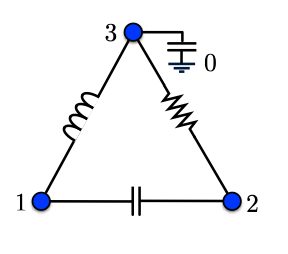
\includegraphics[scale=1]{figs/pn1}
\caption{\label{fig:pn1}sds}
\end{figure}

\end{example}
\begin{figure}
\centering
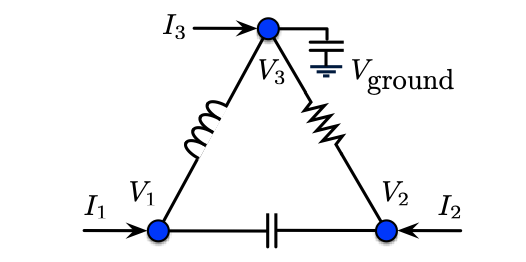
\includegraphics[scale=1]{figs/pn2}
\caption{\label{fig:pn2}sds}
\end{figure}
The basic physical variables are the voltages and currents. On each node we have a potential and a current injection and on each edge we have voltage and current flows. The voltage is a complex number $V=Ee^{i\theta}$ with voltage magnitue and voltage angles.  In Figure \ref{fig:pn2} we see the three external injections $I_1,I_2,I_3$, the three voltage potentials $V_1,V_2,V_3$ and the reference $V_{ground}=0V$. The fundamental equations describing an AC circuit are 
\begin{itemize}
\item Ohm's law  $I_{i\rightarrow j}=\frac{1}{Z_{ij}}(V_i-V_j)$
\item Kirchhoffs current law: $I_i+\sum_j I_{j\rightarrow i}=0$
\item current balance equations $I_i=-\sum_jI_{j\rightarrow i}=\sum_j \frac{1}{Z_{ij}}(V_i-V_j)=\sum_j Y_{ij}V_j$ or $I=Y\cdot V$
\item complex power $S=V_i\bar{I}_i=P+iQ$
\end{itemize}

The power balance equations are formed by setting power injection equal to the sum of the power flows. This leads to
$S_i=V_i\bar{I}_i=\sum_j V_i\bar{Y}_{ij}\bar{V}_j$. Inserting the polar form for $V$ and separating by real and imaginary part we get the power flow equation.
\begin{definition}
Let $G=(V,E)$ be a graph representing the power grid. On each node $i\in V$ a complex voltage $E_ie^{i\theta_i}$ and a complex power $S_i=P_i+iQ_i$ is defined. The AC Power Flow balance equations are given by 
\begin{align}
P_i&=\sum_j B_{ij}E_iE_j\sin{\theta_i-\theta_j}+G_{ij}E_iE_j\cos{\theta_i-\theta_j}\forall i,j\in V\\
Q_i&=\sum_j- B_{ij}E_iE_j\cos{\theta_i-\theta_j}+G_{ij}E_iE_j\sin{\theta_i-\theta_j} \forall i,j\in V
\end{align}

\end{definition}
The power flow equations are a set of $2*N$ real equations, where $N$ is the number of buses on $2*N$ complex variables, which are $4*N$ real variables. This means that we have more variables than equations. However typical buses are modelled as either loads or synchronous generators. Loads have given active power and reactive power and generators have given constant power and voltage magnitude meaning we distiguish between $PQ$ buses and $PV$ buses. There is also the notion of a slack bus where $E$ and $\theta$ are specified. 
\subsection{Physical Units}
Active power (P) is measured in Watt (W) which in SI units is $\frac{kg \;m^2}{s^3}\frac{J}{s}$. Complex Power(S), measured in the same SI units,  is  called volt-ampere and can be a complex number $S=P+iQ$ and $Q$ is the reactive power which is such that $iQ$ is measured in volt-ampere and therefore $Q$ is measuerd in volt-ampere reactive (VAR). Reactive power exists in an AC circuit when the current and voltage are not in phase. The term VAR was proposed by the Romanian electrical engineer Constantin Budeanu and introduced in 1930 by the IEC in Stockholm, which has adopted it as the unit for reactive power. Special instruments called varmeters are available to measure the reactive power in a circuit. Voltage is measured in Volt which is $\frac{kg\; m^2}{As^3}$ in SI units. Current is measured in Ampere $A$,  which means that if we multiply Volt with Ampere we get Watt. The unit of impedance is Ohm which is $\frac{V}{A}=\frac{kg\; m^2}{A^2s^3}$.

